\vspace{-1em}
\begin{figure}[!htbp]
    \centering
    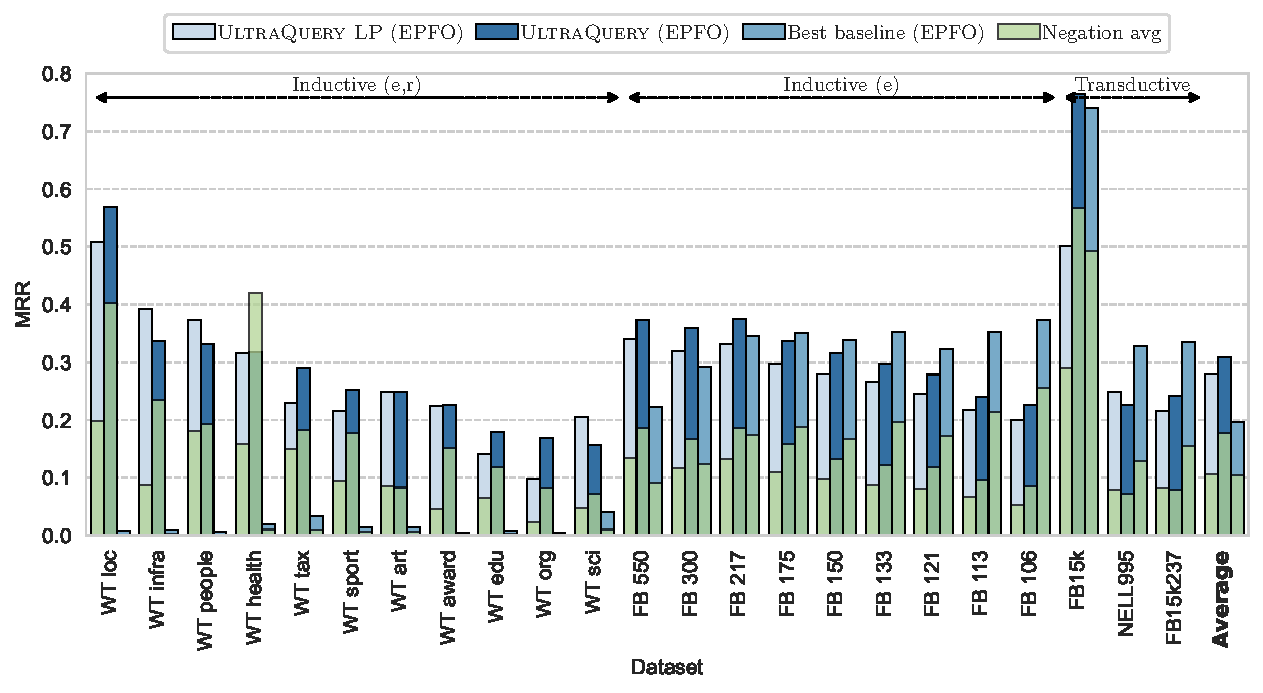
\includegraphics[width=\linewidth]{figs/mainfig1_MRR_pyg.pdf}
    \vskip -0.12 in
    \caption{Zero-shot query answering performance (MRR, higher is better) of a single \method model trained on one FB15k237 queries dataset compared to the best available baselines and ablated \methodlp on 23 datasets. \emph{EPFO} is the average of 9 query types with $(\wedge, \lor)$ operators, \emph{Negation} is the average of 5 query types with the negation operator $(\neg)$. %-- trainable for each transductive and inductive $(e)$ dataset, and the heuristic baseline for newly introduced inductive $(e,r)$ datasets. 
    %\methodlp is an ablated version trained only on \emph{1p} link prediction. 
    On average, a single \method model outperforms the best baselines trained specifically on each dataset. More results are presented in Table~\ref{tab:maintab1} and Appendix~\ref{app:more_results}.
    }
    \label{fig:main_fig1}
\end{figure}

\section{Introduction}
\label{sec:intro}

\begin{wrapfigure}{R}{0.5\textwidth}
\begin{minipage}{0.5\textwidth}
\vspace{-1em}
    %\begin{figure}
        \centering
        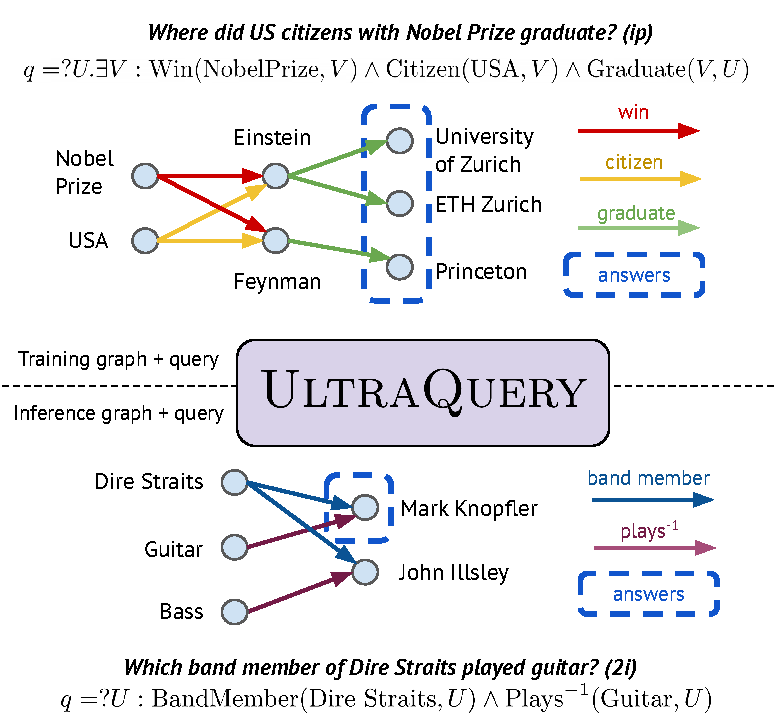
\includegraphics[width=\textwidth]{figs/UltraQuery_Fig1.pdf}
        %\vspace{-2em}
         \vskip -0.1in
        \caption{The inductive logical query answering setup where training and inference graphs (and queries) have different entity and relation vocabularies. We propose a single model (\method) that zero-shot generalizes to query answering % against any unseen
    on any graph with new entity or relation vocabulary at inference time.}
        \label{fig:intro}
    %\end{figure}
    %\vskip -0.2in
    \vspace{-1em}
\end{minipage}
\end{wrapfigure}

Complex logical query answering (\clqa) generalizes simple knowledge graph (KG) completion to more complex, compositional queries with logical operators such as intersection $(\wedge)$, union $(\lor)$, and negation $(\lnot)$.
Such queries are expressed in a subset of first-order logic (FOL) where existentially quantified $(\exists)$ \emph{variables} and given \emph{constants} comprise \emph{relation projections} (or \emph{atoms}), and logical operators combine projections into a logical query (graph pattern). 
A typical example of a logical query~\citep{ren2023ngdb} is presented in \autoref{fig:intro}: $?U.\exists V : \texttt{Win}(\texttt{NobelPrize}, V) \land \texttt{Citizen}(\texttt{USA}, V) \land \texttt{Graduate}(V, U)$ where $\texttt{Win}()$ is a relation projection, $\texttt{NobelPrize}$ is a constant, and $V$ is an existentially quantified variable.




% \begin{figure}[t]
%     \centering
%     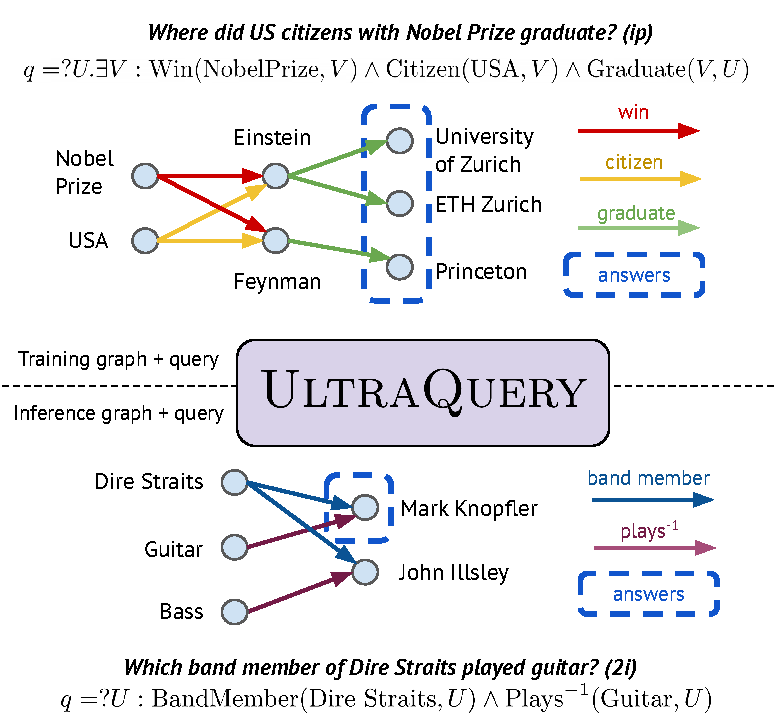
\includegraphics[width=0.5\columnwidth]{figs/UltraQuery_Fig1.pdf}
%     \vskip -0.1in
%     \caption{The inductive logical query answering setup where training and inference graphs (and queries) have different entity and relation vocabularies. We propose a single model (\method) that zero-shot generalizes to query answering % against any unseen
%     on any graph with new entity or relation vocabulary at inference time. \mg{wrapfig it into the first paragraph}}
%     \label{fig:intro}
%     \vskip -0.2in
% \end{figure}

% \clqa assumes that underlying KGs are incomplete such that the projection operator has to predict missing edges and reach the answers unobtainable by simple graph traversal.
Due to the incompleteness of most KGs, these logical queries cannot be directly solved by graph traversal algorithms. Consequently, \clqa methods have to deal with missing edges when modeling the projection operators.
The vast majority of existing \clqa methods~\citep{ren2023ngdb,q2b,betae,cqd,qto} % can only
predict missing edges by learning graph-specific entity and relation embeddings making such approaches transductive and not generalizable to other KGs. 
A few approaches~\citep{gnn_qe,galkin2022,sheaves} are able to generalize query answering to new nodes at inference time but still need a fixed relation vocabulary.

In this work, we focus on the hardest inductive generalization setup where queries and underlying graphs at inference time are completely different from the training graph, \ie, both entities and relations are new.   
Furthermore, we aim at performing \clqa in the \emph{zero-shot} setting with one single model. That is, instead of %training every model on each target dataset,
%adaptively 
finetuning a model on each target dataset,
we seek to design a unified approach that generalizes to any KG and %any complex 
query at inference time.
For example, in \autoref{fig:intro}, the training graph describes academic entities with relations \texttt{Win}, \texttt{Citizen}, \texttt{Graduate}\footnote{We assume the presence of respective inverse relations $\texttt{r}^{-1}$.} whereas the inference graph describes music entities with relations \texttt{Band Member} and \texttt{Plays}. 
The query against the inference graph $?U:\texttt{BandMember}(\texttt{Dire Straits}, U) \wedge \texttt{Plays}^{-1}(\texttt{Guitar}, U)$ involves both new entities 
%(\texttt{Dire Straits}, \texttt{Guitar}) 
and relations 
%(\texttt{Band Member}, \texttt{Plays}) 
and, to the best of our knowledge, cannot be tackled by any existing \clqa method that learns a fixed set of entities or relation embeddings from the training graph.

\textbf{Contributions.} 
Our contributions are two-fold. First, none of the existing \clqa methods can generalize to query answering over new arbitrary KGs with new entities and relations at inference time. 
We bridge this gap by leveraging the recent progress in inductive KG reasoning~\citep{ultra,isdea} and devise \method, the first %\clqa approach 
foundation model for \clqa that generalizes to logical queries on any arbitrary KG with any entity and relation vocabulary in the zero-shot fashion without relying on any external node or edge features. 
%\method follows the blueprint of GNN-QE~\citep{gnn_qe} with the  projection operator parameterized by a graph neural network (GNN) and non-parametric logical operators implemented with fuzzy logics~\citep{vankrieken_fuzzy}.
\method parameterizes the projection operator by an inductive graph neural network (GNN) and implements non-parametric logical operators with fuzzy logics~\citep{vankrieken_fuzzy}.
The pre-trained projection operator~\citep{ultra} does not learn any graph-specific entity nor relation embeddings thanks to the % transferable
generalizable meta-graph representation of relation interactions, and %is therefore zero-shot transferable to any KG.
therefore enables zero-shot generalization to any KG.

% Elaborate more on UltraQuery?

% Experimental evidence
% Furthermore,
Second, in the absence of existing datasets for our inductive generalization setup,
we curate a novel suite of 11 inductive query answering datasets where graphs and queries at inference time  have new entity and relation vocabularies.
Experimentally, we train a single \method model on one dataset and probe on other 22 transductive and inductive datasets.
Averaged across the datasets, a single \method model outperforms by 50\% (relative MRR) the best reported baselines in the literature (often tailored to specific graphs) on both EPFO queries and queries with negation.
